\section {Video Selfie}
The first question we ask about this dataset, to understand the contribution of human affects was, is there any such thing as a video selfie. To understand this better, we processed each video using the well known framework for face detection by Viola and Jones \cite{Viola:2004:RRF:966432.966458} to detect profile and frontal faces in a video. We collected these measurements across all the collected vine videos and found that more than 50 percent of popular vines which ranked in top 100 that day, had more than 50 percent of the face to frame ratio. Moreover orientation of faces seemed to be mixed between frontal and side ways. The mean ration of face frames to total frames was 54.74 percent, across the collected samples. This says a lot about the nature of this social media. There seems to be a preference among Vine consumers towards videos with obvious face protagonist over others. 

\begin{figure}
\centering
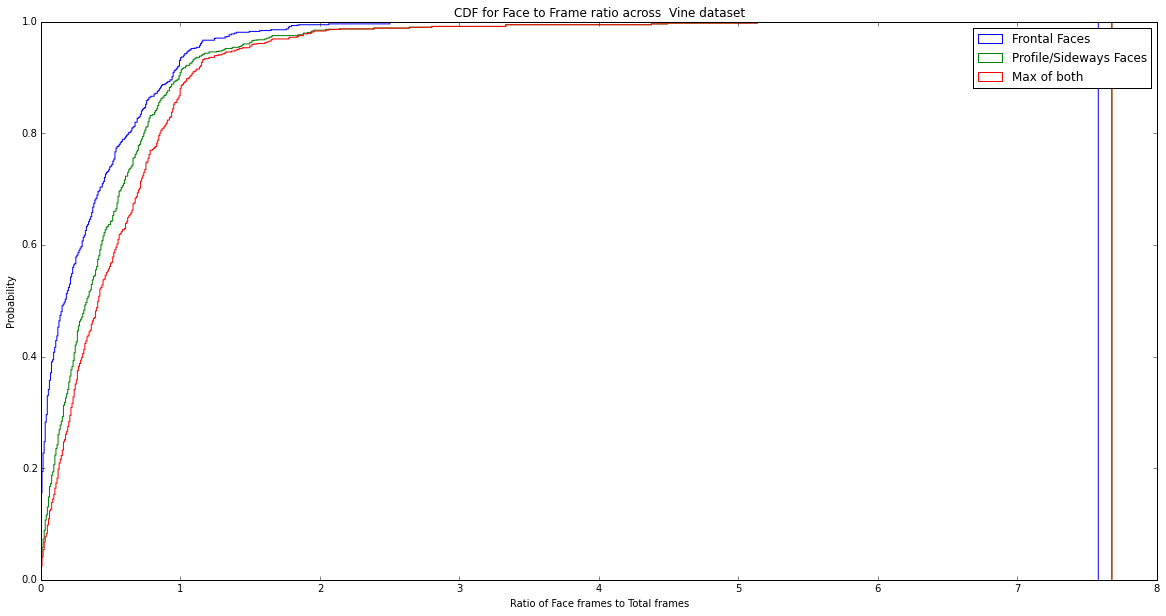
\includegraphics[width=\columnwidth]{plots/CDF_FACE_PROFILE}
\caption{\textbf{CDF of ration if Face frames to total frames in a Vine video.}}
\label{fig:Like_Repost_CDF}
\end{figure}
